\documentclass{beamer}
%\documentclass[notes]{beamer}

\usepackage[T1]{fontenc}
\usepackage[utf8]{inputenc}
\usepackage{default}
\usepackage{listings}
\usepackage{fancybox}
\usepackage{xcolor}
\usepackage{tikz}
\usetikzlibrary{arrows,positioning,calc,shapes.geometric}
\usepackage{mathtools}
\usepackage[normalem]{ulem}
%\usepackage{usenames, dvipsnames}{color}
\usepackage{subfigure}
\usepackage{graphicx}
\usepackage{url}
\usepackage{pbox}
\usepackage{amsmath}
\usepackage{amsthm}
\usepackage{amssymb}

\definecolor{keywordcolor}{rgb}{0.7, 0.1, 0.1}   % red
\definecolor{tacticcolor}{rgb}{0.1, 0.2, 0.6}    % blue
\definecolor{commentcolor}{rgb}{0.4, 0.4, 0.4}   % grey
\definecolor{symbolcolor}{rgb}{0.0, 0.1, 0.6}    % blue
\definecolor{sortcolor}{rgb}{0.1, 0.5, 0.1}      % green

\usepackage{listings}
\def\lstlanguagefiles{lstlean.tex}
\lstset{language=lean}
\usepackage{textcomp}

\title [Automation and Computation in Lean]{Automation and Computation in the Lean Theorem Prover}
%\subtitle{A Heuristic Procedure for Reasoning with Real Inequalities}

%\author [R.\ Y.\ Lewis]{Robert Y. Lewis\\[3mm]{\footnotesize Joint work with Jeremy Avigad and Cody Roux}}
\author [R.\ Y.\ Lewis, L. de Moura]{Robert Y.\ Lewis\inst{1} \and Leonardo de Moura\inst{2}}
\institute[CMU; MSR]{\inst{1}Carnegie Mellon University \and \inst{2}Microsoft Research, Redmond}
\date{April 6, 2016}

%\date{}

%\usetheme{Malmoe}
%\usetheme{AnnArbor}
%\usecolortheme{beaver}
\setbeamercolor{block title}{fg=white,bg=blue}%{fg=white,bg=red!75!black}
\setbeamercolor{block body}{fg=white,bg=gray!75!black}

\setbeamercolor{title}{bg=gray!155!black}

\newcommand{\RR}{\mathbb{R}}
\newcommand{\QQ}{\mathbb{Q}}
\newcommand{\ZZ}{\mathbb{Z}}
\newcommand{\NN}{\mathbb{N}}

\newcommand{\fn}[1]{\text{#1}}
\newcommand{\inv}{^{-1}}

\begin{document}

\frame{\titlepage}

%\begin{frame}
 %\frametitle{Table of Contents}
 %\tableofcontents
%\end{frame}

\begin{frame}
\frametitle{Goals for this talk}
\begin{itemize}
\item Introduce Lean: a new proof assistant based on dependent type theory
\item Discuss the current state of, and future prospects for, automation in Lean
\item Introduce Polya: a system for verifying real nonlinear inequalities
\end{itemize}

\end{frame}

\begin{frame}
\frametitle{Credit to...}
\begin{itemize}
\item Leonardo de Moura
\item Soonho Kong, Floris van Doorn, Daniel Selsam
\item Jeremy Avigad, Cody Roux
\item Many others....
\end{itemize}

\end{frame}


\note[itemize]{
\item Leonardo de Moura: lead developer of Lean
\item Soonho Kong, Floris van Doorn, Daniel Selsam, and others: contributors to library and system
\item Jeremy Avigad: Lean standard library and Polya
\item Cody Roux: contributions to Polya
}

\begin{frame}
\frametitle{Lean details}
\begin{itemize}
\item Open source
\item Constructive dependent type theory
\item Designed with automation in mind
\begin{itemize}
\item Interactive theorem prover with strong automation
\item Automated theorem prover with verified mathematical library
\end{itemize}
\item ``Standard'' and ``homotopy type theory'' flavors
\begin{itemize}
\item Standard: proof-irrelevant, impredicative Prop, classical logic available, quotient types
\item HoTT: proof-relevant, no impredicative Prop, univalence, HIT
\end{itemize}
\item Seamlessly integrate classical reasoning
\end{itemize}

\end{frame}

\begin{frame}
\frametitle{Lean details}

\begin{itemize}
\item Small kernel
\begin{itemize}
\item No termination checker, pattern matching, etc.
\end{itemize}
\item Reference type checker
\item Mixed tactic and declarative proof styles
\item Powerful elaborator with strong type class inference mechanism
\item May see similarities to other systems: not surprising

\vspace{.5cm}

\item Very young system!
\end{itemize}

\end{frame}

\begin{frame}
 \frametitle{Lean details}
 The standard library already has:
\begin{itemize}
 \item datatypes: booleans, lists, tuples, finsets, sets
 \item number systems: nat, int, rat, real, complex
 \item the algebraic hiearachy, through ordered fields
 \item ``big operations'': finite sums and products, etc.
 \item elementary number theory (e.g.~primes, gcd's, unique factorization, etc.)
 \item elementary set theory
 \item elementary group theory (Sylow's theorem)
 \item beginnings of analysis: topological spaces, limits, continuity, the intermediate value theorem
\end{itemize}
\end{frame}

\begin{frame}{Lean details}
 
Currently working on:
\begin{itemize}
 \item topology (connectedness, compactness)
 \item linear algebra
 \item analysis: transcendental functions, the Frechet derivative
 \item measure theory (Lebesgue integration)
 \item group theory %(including geometric group theory)
% \item homological algebra (in support of the spectral project)
\end{itemize}

\end{frame}

%\begin{frame}[fragile]
%\frametitle{Computable definitions}
%
%Lean allows you to integrate classical and constructive reasoning, and keeps track of which definitions are computable.
%
%\begin{lstlisting}
%definition map (f : A $\to$ B) : list A $\to$ list B
%| []       := []
%| (a :: l) := f a :: map l
%
%noncomputable definition inv_fun (f : X $\to$ Y) 
%  (a : set X) (dflt : X) (y : Y) : X :=
%if H : $\exists_0$ x $\in$ a, f x = y then some H else dflt
%
%definition add (x y : $\RR$) : $\RR$ := ...
%                       
%noncomputable definition div (x y : $\RR$) : $\RR$ := 
%x * y$^{-1}$
%
%\end{lstlisting}
%
%\end{frame}
%
%\begin{frame}
%\frametitle{Computable definitions}
%\begin{itemize}
%\item Much of the core library is constructive
%\item The reals constructively form an ordered ring
%\item Topology, analysis, etc are classical
%\item Finite sets are developed classically and constructively 
%\end{itemize}
%
%\end{frame}


\begin{frame}[fragile]
\frametitle{Example}
\begin{lstlisting}[basicstyle=\small]
definition infinite_primes (n : nat) : {p | p $\ge$ n $\wedge$ prime p} :=
let m := fact (n + 1) in
have m $\ge$ 1,     from le_of_lt_succ (succ_lt_succ (fact_pos _)),
have m + 1 $\ge$ 2, from succ_le_succ this,
obtain p `prime p` `p | m + 1`, from sub_prime_and_dvd this,
have p $\ge$ 2,     from ge_two_of_prime `prime p`,
have p > 0,     from lt_of_succ_lt (lt_of_succ_le `p $\ge$ 2`),
have p $\ge$ n,     from by_contradiction
  (suppose $\neg$ p $\ge$ n,
    have p < n,   from lt_of_not_ge this,
    have p $\le$ n + 1, from le_of_lt (lt.step this),
    have p | m,    from dvd_fact `p > 0` this,
    have p | 1,    from 
            dvd_of_dvd_add_right (!add.comm $\triangleright$ `p | m + 1`) this,
    have p $\le$ 1,   from le_of_dvd zero_lt_one this,
    absurd (le.trans `2 $\le$ p` `p $\le$ 1`) dec_trivial),
subtype.tag p (and.intro this `prime p`)
\end{lstlisting}
\end{frame}

\note[itemize]{
\item This slide shows off the declarative style
\item Note that {\tt by contradiction} is inferring the decidability of $\ge$ on $\NN$.
}

\begin{frame}
\frametitle{Type class inference}
\begin{itemize}
\item Can declare \alert{classes} and \alert{instances}
\item Variables marked with [ ] are inferred by searching for instances of the correct types
\item Search is recursive and backtracking and caches aggressively
\end{itemize}

\end{frame}


\begin{frame}[fragile]
\frametitle{Type class inference}
\begin{lstlisting}[basicstyle=\footnotesize]
inductive inhabited [class] (A : Type) : Type :=
mk : A $\to$ inhabited A

definition default (A : Type) [h : inhabited A] : A :=
inhabited.rec ($\lambda$ a, a) h

definition prop_inhabited [instance] : inhabited Prop :=
inhabited.mk true

definition fun_inhabited [instance]
      (A B : Type) [h : inhabited B] : inhabited (A $\to$ B) :=
inhabited.mk ($\lambda$ x : A, default B)

definition prod_inhabited [instance]
      (A B : Type) [ha : inhabited A] [hb : inhabited B] : inhabited (A $\times$ B) :=
inhabited.mk (default A, default B)

eval default (nat $\to$ nat $\times$ Prop)
-- $\lambda$ (a : nat), (0, true)
\end{lstlisting}
\end{frame}

\note[itemize]{
\item We define a class {\tt inhabited} and atomic instances {\tt prop inhabited} and {\tt nat inhabited}.
\item Then compound instances are defined.
\item Evaluating {\tt default} traces through the instances to synthesize a term of the correct type.
}

\begin{frame}[fragile]
\frametitle{Algebraic hierarchy}
Type class inference lets us construct the algebraic hierarchy in a uniform way.
\begin{lstlisting}[basicstyle=\footnotesize]
structure semigroup [class] (A : Type) extends has_mul A :=
(mul_assoc : $\forall$ a b c, mul (mul a b) c = mul a (mul b c))

structure monoid [class] (A : Type) extends semigroup A, has_one A :=
(one_mul : $\forall$ a, mul one a = a) (mul_one : $\forall$ a, mul a one = a)

structure group [class] (A : Type) extends monoid A, has_inv A :=
(mul_left_inv : $\forall$ a, mul (inv a) a = one)

theorem inv_mul_cancel_left {A : Type} [H : group A] (a b : A) : 
              a$\inv \cdot$ (a $\cdot$ b) = b :=
  by rewrite [-mul.assoc, mul.left_inv, one_mul]
  
structure linear_ordered_field [class] (A : Type) extends linear_ordered_ring A, field A
\end{lstlisting}

\end{frame}

\note[itemize]{
\item Lots of structures left out of this list, for room
\item {\tt structure} is shorthand for an inductive type with one constructor.
\item Defining a structure with {\tt extends} automatically defines instances to the smaller class.
\item So using {\tt mul.assoc} in {\tt inv mul cancel left} finds the {\tt mul.assoc} defined on semigroups.
}

\begin{frame}[fragile]
\frametitle{Algebraic hierarchy}
\begin{lstlisting}[basicstyle=\footnotesize]
structure left_module [class] (R M : Type) [ringR : ring R]
  extends has_scalar R M, add_comm_group M :=
(smul_left_distrib : $\forall$ (r : R) (x y : M), 
   smul r (add x y) = (add (smul r x) (smul r y)))
(smul_right_distrib : $\forall$ (r s : R) (x : M), 
   smul (ring.add r s) x = (add (smul r x) (smul s x)))
(mul_smul : $\forall$ r s x, smul (mul r s) x = smul r (smul s x))
(one_smul : $\forall$ x, smul one x = x)

definition m_left_module [instance] (A : Type) [ring A] (m n : $\NN$) : 
                left_module A (matrix A m n) := ...
\end{lstlisting}
\end{frame}

\begin{frame}
 \frametitle{Algebraic hierarchy}
 The standard library has 
\begin{itemize}
 \item order structures (including lattices, complete lattices)
 \item additive and multiplicative semigroups, monoids, groups, \ldots
 \item rings, fields, ordered rings, ordered fields, \ldots
 \item modules over arbitrary rings, vector spaces, normed spaces, \ldots
 \item homomorphisms preserving appropriate parts of structures
\end{itemize}
\end{frame}


\begin{frame}[fragile]
\frametitle{Concrete number structures}
When types instantiate these algebraic structures, all theorems proved in the general case are immediately available in the concrete setting.

\begin{onlyenv}<1>
\begin{lstlisting}[basicstyle=\footnotesize]
definition real_ord_ring [reducible] [instance] : ordered_ring $\RR$ :=
{ ordered_ring, real.comm_ring,
  le_refl := real.le_refl,
  le_trans := @real.le_trans,
  mul_pos := real.mul_pos,
  mul_nonneg := real.mul_nonneg,
  zero_ne_one := real.zero_ne_one,
  add_le_add_left := real.add_le_add_left,
  le_antisymm := @real.eq_of_le_of_ge,
  lt_irrefl := real.lt_irrefl,
  lt_of_le_of_lt := @real.lt_of_le_of_lt,
  lt_of_lt_of_le := @real.lt_of_lt_of_le,
  le_of_lt := @real.le_of_lt,
  add_lt_add_left := real.add_lt_add_left
}
\end{lstlisting}
\end{onlyenv}

\begin{onlyenv}<2>
\begin{lstlisting}[basicstyle=\footnotesize]
theorem translate_cts {f : $\RR \to \RR$} (Hcon : continuous f) (a : $\RR$) :
        continuous ($\lambda$ x, (f x) + a) :=
  begin
    intros x $\epsilon$ H$\epsilon$,
    cases Hcon x H$\epsilon$ with $\delta$ H$\delta$,
    cases H$\delta$ with H$\delta_1$ H$\delta_2$,
    existsi $\delta$,
    split,
    assumption,
    intros x' Hx',
    rewrite [add_sub_comm, sub_self, add_zero],
    apply H$\delta_2$,
    assumption
  end
\end{lstlisting}
\end{onlyenv}

\end{frame}

\begin{frame}[fragile]
\frametitle{Numeral computation}
Binary numerals can be used in Lean in any structure that has 0, 1, and +. 

\begin{lstlisting}[basicstyle=\footnotesize]
definition bit0 {A : Type} [s : has_add A]  (a  : A) : A := add a a
definition bit1 {A : Type} [s : has_one A] [t : has_add A] (a : A) : A := add (bit0 a) one
\end{lstlisting}

\vspace{.5em}

With the right instances present, numerical simplification can be done efficiently in an arbitrary type using binary arithmetic.

%\vspace{-.5em}
\begin{lstlisting}[basicstyle=\footnotesize]
example : 1900 + 220*4 = (2780 : $\NN$) :=
  by norm_num

example : (253 + 5 * 10) / 3 = (101 : $\RR$) :=
  by norm_num
     
example (A : Type) [linear_ordered_field A] : (11 + 25) / 8 = (9 : A) / 2
  := by norm_num
\end{lstlisting}

\end{frame}

\begin{frame}
\frametitle{Upshots for automation}
This uniform development is helpful for automation.

\begin{itemize}
\item Theorems are not duplicated, so strategies apply across structures.
\item Numerals behave identically, and easy to identify when the necessary properties are present.
\end{itemize}

Present/forthcoming:
\begin{itemize}
\item Term simplifier
\item Fourier-Motzkin linear inequality solver
\item Simplex solver
\item Blast (general purpose auto proof search)
\item Blast (machine learning)
\item Polya: nonlinear inequalities
\end{itemize}

\end{frame}

\begin{frame}
\frametitle{Broader questions}

\begin{itemize}
\item How do we adapt standard proof search techniques to dependent type theory?

\item How can we incorporate AI methods in the short term? Long term?

\end{itemize}

\end{frame}

\note[itemize]{
\item Theorems are not duplicated, so learned strategies apply across structures.
\item Numerals behave identically, and easy to identify when the necessary properties are present.
\item Term simplifier: present
\item FM linear arithmetic: waiting to be integrated
\item Simplex solver: in progress
\item Blast: partially implemented
\item Machine learning: coming eventually
}

\begin{frame}
\frametitle{Polya}
\alert{Polya}: a tool for heuristically verifying real-valued inequalities over extensions of RCF
\begin{itemize}
\item Lightweight
\item Flexible, extensible
\item ``Reasonably'' constructive
\item NOT a decision procedure
\item Avigad, Lewis, Roux. \emph{A heuristic prover for real inequalities} (2014)
\end{itemize}
\end{frame}

\begin{frame}
 \frametitle{A motivating example}
 \begin{align*}
  0 < x < y,\ u & < v \\
  \implies & \\
  2u + \text{exp}&(1 + x + x^4) < 2v + \text{exp}(1 + y + y^4)
 \end{align*}
 
 \begin{itemize}
  \item This inference is not contained in linear arithmetic or real closed fields.
  \item This inference is tight: symbolic or numeric approximations to exp are not useful.
  \item {Backchaining} using monotonicity properties suggests many equally plausible subgoals.
  \item But, the inference is completely straightforward.
 \end{itemize}
 \end{frame}

\begin{frame}
 \frametitle{A new method}
 We propose and implement a method based on this type of heuristically guided forward reasoning. Our method:
 
 \begin{itemize}
  \item Verifies inequalities on which other procedures fail.
  %\item Extends beyond the language of RCF.
  \item Is relatively easy to implement in Lean.
  \item Captures natural, human-like inferences.
  \item Performs well on real-life problems.
  \vspace{.25cm}
  \item Is not complete.
  \item Is not guaranteed to terminate.
 \end{itemize}
 
 We envision it as a complement, not a replacement, to other verification procedures.

\end{frame}

\begin{frame}
\frametitle{Implementations}
\begin{itemize}
\item Python prototype: not proof-producing, but can experiment
\item Lean version: on the way!
\end{itemize}
\end{frame}

\begin{frame}
 \frametitle{Terms and normal forms}
 The inequality 
 $$15 < 3 (3y + 5x + 4 x y)^2 f(u + v)^{-1}$$
 is expressed canonically as
% \only<1>{$$\underbrace{\mathbf{1}}_{t_0} \leq 5 \cdot (\underbrace{x}_{t_1} + \frac{3}{5} \cdot \underbrace{y}_{t_2} + \frac{4}{5} \cdot \underbrace{x y}_{t_3 = t_1 t_2})^2 f(\underbrace{u}_{t_4} + \underbrace{v}_{t_5})^{-1}$$}
% 
% \only<2>{$$\underbrace{\mathbf{1}}_{t_0} \leq 5 \cdot (\underbrace{\underbrace{x}_{t_1} + \frac{3}{5} \cdot \underbrace{y}_{t_2} + \frac{4}{5} \cdot \underbrace{x y}_{t_3 = t_1 t_2}}_{t_6 = t_1 + \frac{3}{5}t_2 + \frac{4}{5}t_3})^2 f(\underbrace{\underbrace{u}_{t_4} + \underbrace{v}_{t_5}}_{t_7 = t_4 + t_5})^{-1}$$}
% 
% \only<3>{$$\underbrace{\mathbf{1}}_{t_0} \leq 5 \cdot (\underbrace{\underbrace{x}_{t_1} + \frac{3}{5} \cdot \underbrace{y}_{t_2} + \frac{4}{5} \cdot \underbrace{x y}_{t_3 = t_1 t_2}}_{t_6 = t_1 + \frac{3}{5}t_2 + \frac{4}{5}t_3})^2 \underbrace{f(\underbrace{\underbrace{u}_{t_4} + \underbrace{v}_{t_5}}_{t_7 = t_4 + t_5}}_{t_8 = f(t_7)})^{-1}$$}
% 
% \only<4>{$$\underbrace{\mathbf{1}}_{t_0} \leq 5 \cdot \underbrace{(\underbrace{\underbrace{x}_{t_1} + \frac{3}{5} \cdot \underbrace{y}_{t_2} + \frac{4}{5} \cdot \underbrace{x y}_{t_3 = t_1 t_2}}_{t_6 = t_1 + \frac{3}{5}t_2 + \frac{4}{5}t_3})^2 \underbrace{f(\underbrace{\underbrace{u}_{t_4} + \underbrace{v}_{t_5}}_{t_7 = t_4 + t_5}}_{t_8 = f(t_7)})^{-1}}_{t_9 = t_6^2t_8^{-1}}$$}

  {$$\underbrace{\underbrace{\mathbf{1}}_{t_0} < 5 \cdot \underbrace{(\underbrace{\underbrace{x}_{t_1} + \frac{3}{5} \cdot \underbrace{y}_{t_2} + \frac{4}{5} \cdot \underbrace{x y}_{t_3 = t_1 t_2}}_{t_6 = t_1 + \frac{3}{5}t_2 + \frac{4}{5}t_3})^2 \underbrace{f(\underbrace{\underbrace{u}_{t_4} + \underbrace{v}_{t_5}}_{t_7 = t_4 + t_5}}_{t_8 = f(t_7)})^{-1}}_{t_9 = t_6^2t_8^{-1}}}_{t_0 \leq 5t_9}$$}
 \end{frame}

\note[itemize]{
\item First the term is put in a normal form, with terms arranged alphabetically and constants factored.
\item Then subterms are named. Names are given to problem variables, sums of terms, products of terms, and functions applied to terms.
}

\begin{frame}
 \frametitle{Modules and database}
 Any comparison between canonical terms can be expressed as $t_i \bowtie 0$ or $t_i \bowtie c \cdot t_j$, where $\bowtie\ \in\{ =, \neq, <, \leq, >, \geq \}$. This is in the {common language} of addition and multiplication.
 
 \vspace{.5cm}
 
 A central database (the {blackboard}) stores term definitions and comparisons of this form.
 
 \vspace{.5cm}
 
 {Modules} use this information to learn and assert new comparisons.
 
 \vspace{.5cm}
 
 The procedure has succeeded in verifying an implication when modules assert contradictory information.
\end{frame}

\begin{frame}
 \frametitle{Arithmetic modules}
 If we restrict out attention to atomic comparisons and only additive (or only multiplicative) definitions, then linear methods can be used.
 
 \vspace{.5cm}
 
 Given additive equations $\{t_i = \sum_j c_j \cdot t_{k_j}\}$ and atomic comparisons $\{t_i \bowtie c \cdot t_j\}$ and $\{t_i \bowtie 0\}$, want to saturate the blackboard with the strongest implied atomic comparisons. Two methods:
 
 \begin{itemize}
  \item Fourier-Motzkin elimination
  \item Geometric techniques
 \end{itemize}
 
 The geometric method scales better, but the two methods have the same output.
 
 Modulo some concerns about sign information and irrational numbers, we can do the same with multiplicative equations.
\end{frame}

\begin{frame}
 \frametitle{Fourier-Motzkin additive module}
 
 To find comparisons between $t_1$ and $t_2$, \only<1-4>{eliminate $t_3$:}\only<5->{find the strongest pair:}
 \begin{center}

 \begin{tabular}{ccccc}
   {$\begin{aligned}
    \color<2>{red} {3t_1 + 2t_2 - t_3} > &\ \color<2>{red}0 \\
    \color<2>{red}\color<3>{blue}\color<4>{green!75!black} {4t_1 + t_2 + t_3} \geq &\ \color<2>{red}\color<3>{blue}\color<4>{green!75!black}0 \\
    \color<3>{blue}2t_1 - t_2 - 2 t_3 \geq &\ \color<3>{blue}0 \\
    \color<4>{green!75!black}-2t_2 - t_3 >&\ \color<4>{green!75!black} 0 \\
   \end{aligned}$} & \onslide<2->{$\implies$}
   {$\begin{aligned}
   \onslide<2->{
    \color<2>{red} 7t_1 + 3 t_2 >&\ \color<2>{red}0 \\
    }
   \onslide<3->{
    \color<3>{blue} 10 t_1 + t_2 \geq&\ \color<3>{blue} 0 \\
    }
   \onslide<4->{
    \color<4>{green!75!black} 4t_1 - t_2 >&\ \color<4>{green!75!black} 0
    }
   \end{aligned}$}
   &
   \onslide<5->{$\implies$}
   &
   \onslide<5->{$\begin{aligned}
    t_1 >& -\!\frac{3}{7} t_2 \\
    \color<6>{gray!160!black}{t_1 \geq} &\ \color<6>{gray!160!black}{-\frac{1}{10}t_2} \\
    t_1 >&\ \frac{1}{4}t_2
   \end{aligned}$}
 \end{tabular}

 \end{center}
\end{frame} 

\note[itemize]{
\item Fourier Motzkin steps are simple. It's easy to see how this method can be made proof-producing.
}

\begin{frame}
 \frametitle{Geometric additive module}
The equalities and inequalities in the blackboard describe a polyhedron with vertex at the origin, in halfplane representation.  

 \vspace{.4cm}
 
 By projecting this polyhedron to the $t_i t_j$ plane, one can find the strongest implied comparisons between $t_i$ and $t_j$.
 
 \begin{figure}
\centering
\begin{subfigure}%{.45\linewidth}
  \centering
 % 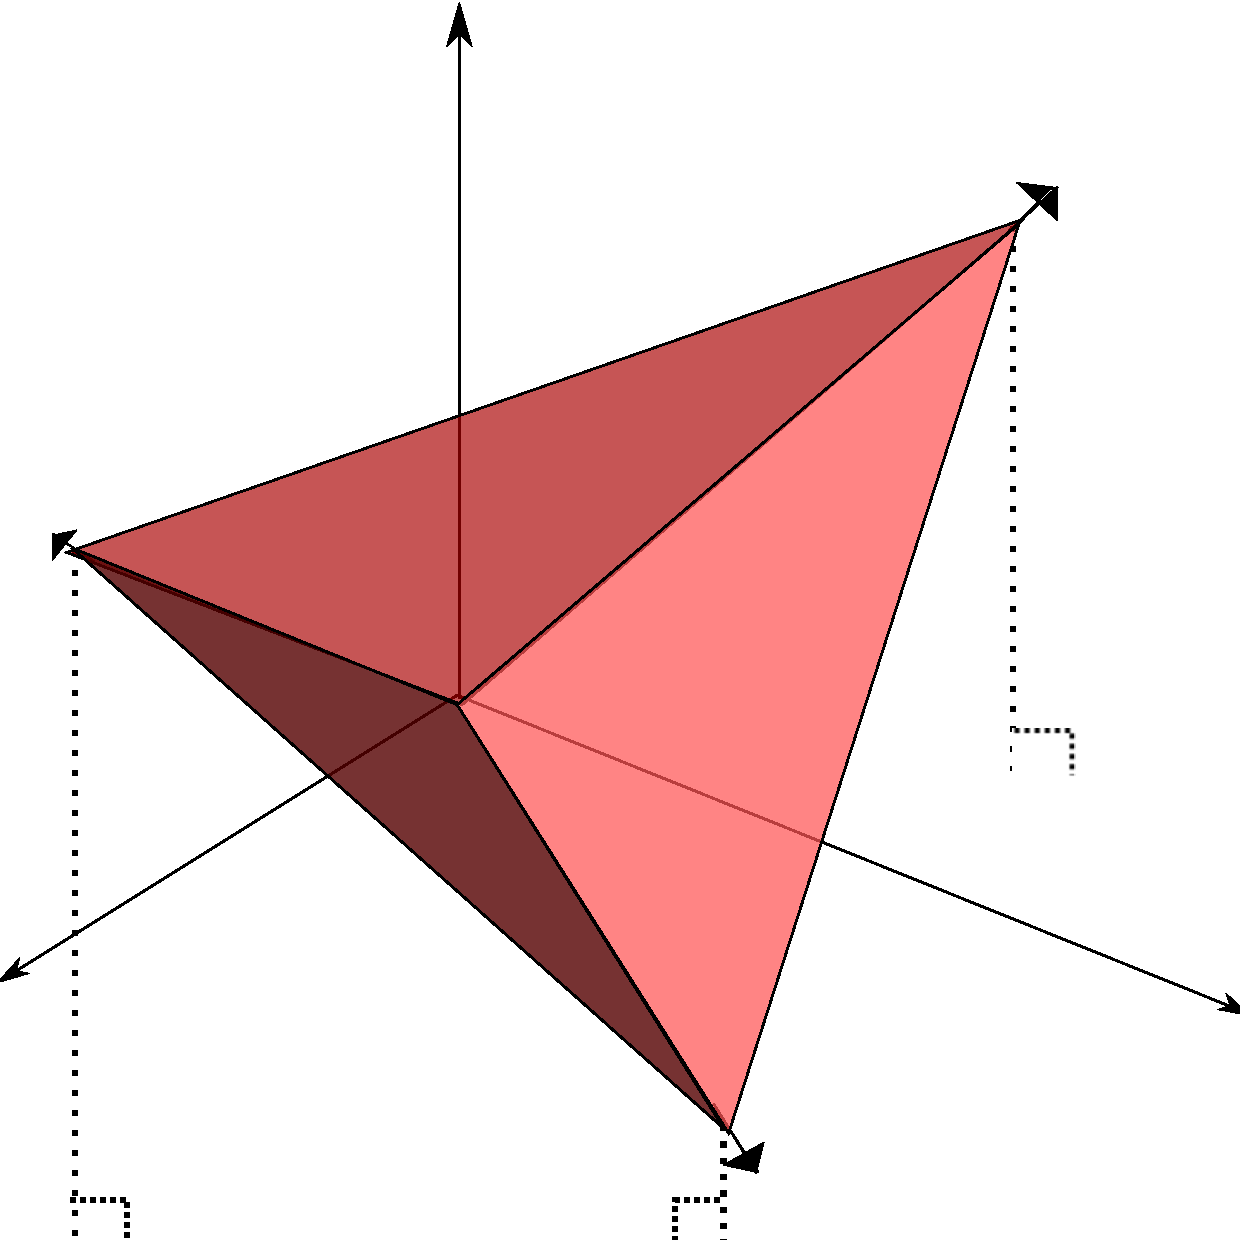
\includegraphics[width=.25\linewidth, bb=0 0 596 596]{3d_poly.pdf_tex}
  \resizebox{.25\linewidth}{.25\linewidth}{\input{3d_poly.pdf_tex}}
\end{subfigure}%
\hspace{.2\linewidth}
\begin{subfigure}%{.45\linewidth}
  \centering
%  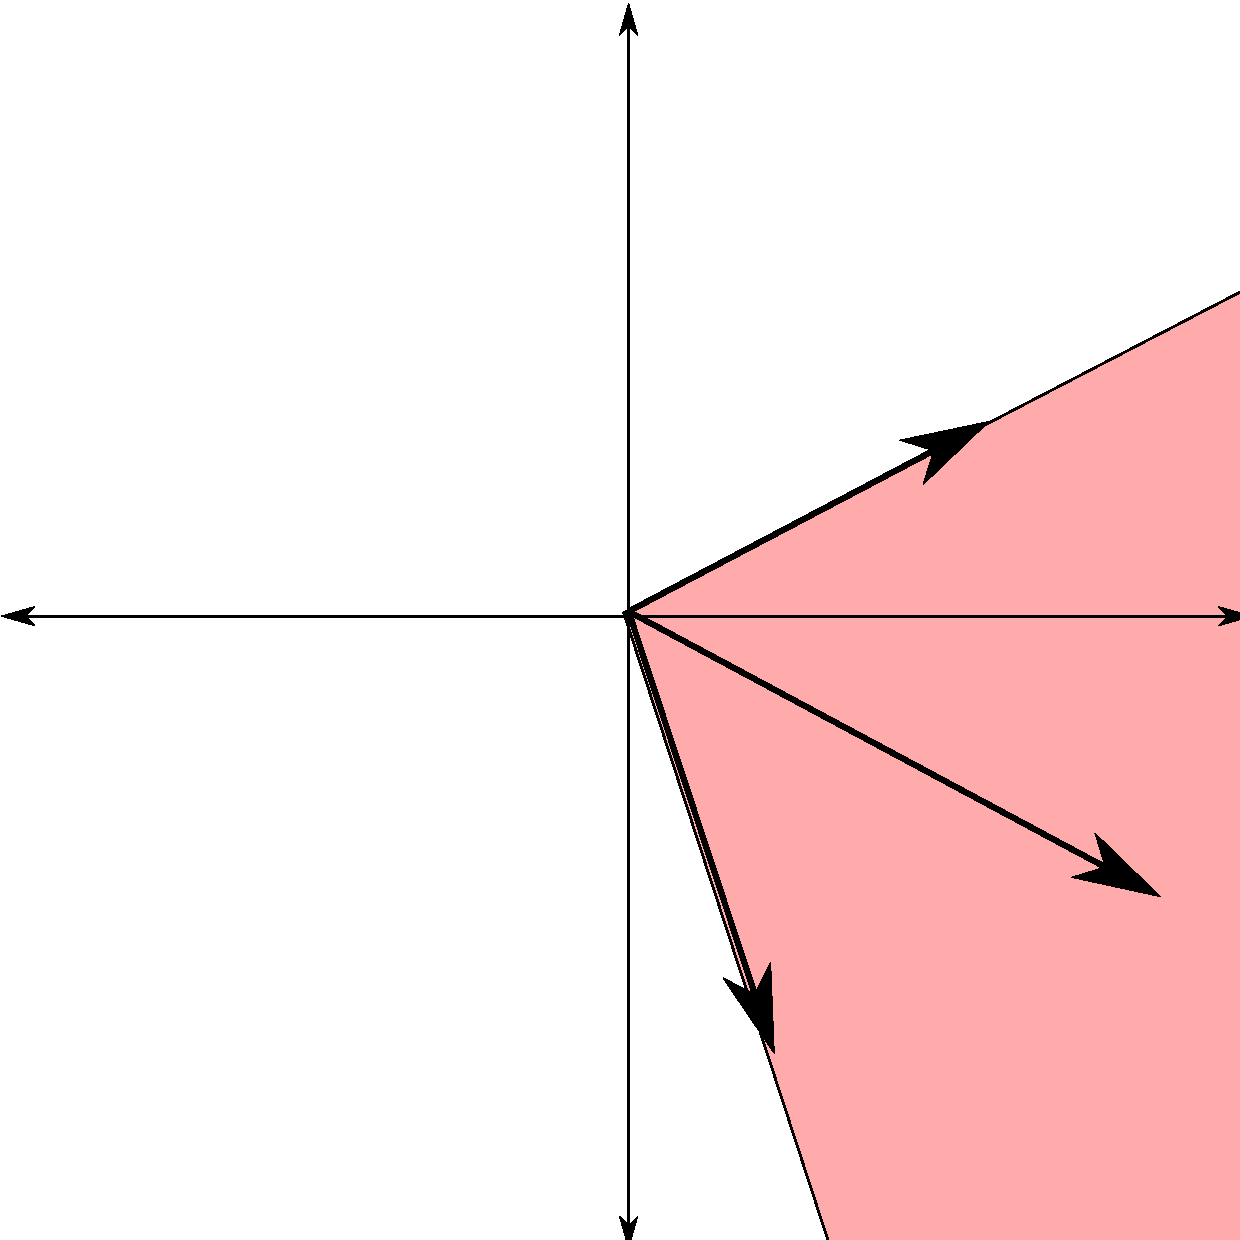
\includegraphics[width=.6\linewidth, bb=0 0 596 596]{2d_proj.pdf_tex}
  \resizebox{.25\linewidth}{.25\linewidth}{\input{2d_proj.pdf_tex}}
 % \def\svgwidth{.6\linewidth}\input{2d_proj.pdf_tex}
% \caption{Projected to the $xy$ plane, the polyhedron implies $x>2y$ and $x>-\frac{1}{3}y$}
 % \caption{Projected to the $xy$ plane, the polyhedron implies $x\geq2y$ and $x\geq-\frac{1}{3}y$}
  \label{fig:geo:projection:b}
\end{subfigure}
%\caption{Variable elimination by geometric projection}
\label{fig:geo:projection}
\end{figure}

 We use the computational geometry packages \alert{cdd} and \alert{lrs} for the conversion from half-plane representation to vertex representation.
 
\end{frame}

\note[itemize]{
\item This approach scales better than the FM method.
\item It's not as clear how to formalize this process.
\item Depends on external packages, which can be buggy.
}

\begin{frame}
\frametitle{Axiom instantiation module}
\begin{itemize}
\item Users can define function terms and axiomatize their behavior.
\begin{itemize}
\item $f$ increasing, positive, etc.
\end{itemize}
\item This module instantiates these axioms heuristically. 
\item Built in handling for min/max, sin/cos, exp/log
\end{itemize}
\end{frame}

\note[itemize] {
\item There's a balance to the instantiation. Too much will slow the process down, too little will miss results.
\item Choices are heuristic, based on unifying ``trigger terms'' from the axioms with terms in the problem.
\item Unification has to happen modulo AC equality (either additively or multiplicatively, not both).
}

\begin{frame}
 \frametitle{Successes}
 Our implementation in Python successfully proves many theorems, some of which are not proved by other systems.
 
 
 \begin{equation}
  0 < x < 1 \implies 1/(1 - x) > 1/(1 - x^2)
 \end{equation}
 
 \begin{equation}
  0 < u, \; u < v, \; 0 < z, \; z + 1 < w  \implies (u + v + z)^3 < (u + v + w)^5
 \end{equation}

 \begin{equation} \begin{split}
  \left(\forall x, y. \; x \leq y \rightarrow f(x) \leq f(y)\right), \; u < v, \;
1 < v, \; x \leq y \implies \\
u + f(x) \leq v^2 + f(y)
\end{split} \end{equation}

\end{frame}

\note[itemize] {
\item Z3 will solve the first two. But in the second, if the exponents are increased, Z3 will slow down and then fail. Polya finds the ``same'' proof no matter what the exponents are.
}

\begin{frame}
 \frametitle{Successes}

  \begin{equation} \begin{split}
  (\forall x, y. \; f(x + y) = f(x) f(y)), \; f(a + b) > 2, \; f(c + d) > 2 \implies \\ f(a + c + b + d) > 4
 \end{split}\end{equation}
 

 \begin{equation}\begin{split}
 0 \le n,\ n < (K / 2) x,\ 0 < c,\ 0 < \epsilon < 1 \implies \\  \left(1 + \frac{\epsilon}{3(C + 3)}\cdot n < K x \right)
 \end{split}\end{equation} 
 
 \begin{equation}
  x < y, \; u \leq v \implies u + \fn{min}(x + 2u, y + 2v) \le x + 3v
 \end{equation}
 
 \begin{equation}
  y > \fn{max}(2, 3x), \; x>0 \implies \fn{exp}(4y - 3x) > \fn{exp}(6) 
 \end{equation}


\end{frame}

\note[itemize] {
\item The first problem involves complicated matching in the unifier.
\item The second comes from Avigad's formalization of the central limit theorem.
}

\begin{frame}
 \frametitle{Limitations}
 Since our method is incomplete, it fails on a wide class of problems where other methods succeed.
 
 \begin{equation}
   x > 0, \; x y z < 0, \; x w > 0 \implies w > yz
 \end{equation}
 
 
  \begin{equation}
  x^2 + 2x + 1 \geq 0
 \end{equation}

 
 \begin{gather}
\begin{split}
  4 \leq x_i \leq &\ 6.3504 \implies \\
    &\ x_1x_4(-x_1 + x_2 + x_3 - x_4 + x_5 + x_6) \\
  &\ + x_2x_5(x_1 - x_2 + x_3 + x_4 - x_5 + x_6) \\
  &\ + x_3x_6(x_1 + x_2 - x_3 + x_4 + x_5 + -x_6) \\
  &\ - x_2x_3x_4 -x_1x_3x_5 - x_1x_2x_6 - x_4x_5x_6 > 0
 \end{split}
 \label{eq:17}
\end{gather}
 


\end{frame}

\begin{frame}
 \frametitle{KeYmaera examples}
 On a collection of 4442 problems generated automatically by KeYmaera, we solve 4255 (96\%) with a 3-second timeout.
 \begin{itemize}
  \item ~8 minutes using geometric packages
 \end{itemize}

 \begin{block}{Example}
  \tt{Hypothesis: ru10**2 == (1/3)*x1u0**2

  Hypothesis: x1u0 <= 0

  Hypothesis: ru10 > 0

  Hypothesis: d1 == -1 * om * (h2 + -1*x2)

  Hypothesis: d2 == om * (h1 + -1*x1)

  Hypothesis: (h1 + -1*x1)**2 + (h2 + -1*x2)**2 == r**2

  Hypothesis: 1 != ru10**-1 * ru10

  Conclusion: False}
 \end{block}

\end{frame}

\begin{frame}{Connections to other systems}
 \begin{itemize}
  \item SMTLIB input
  \item Why3 driver (rudimentary)
 \end{itemize}

\vspace{.5cm}

Lean implementation:
\begin{itemize}
\item Work in progress!
\item Question: how to formalize geometric version?
\end{itemize}
\end{frame}

%\begin{frame}{Broader morals}
%\begin{itemize}
%\item Complete automation in ITP/TT is difficult, but not needed
%\item Small methods to attack subgoals/aid the user are great
%\item What problems can we attack with AI?
%\end{itemize}
%\end{frame}

\begin{frame}
\frametitle{Thanks for listening!}
Lean:
\begin{itemize}
\item \url{http://leanprover.github.io} (interactive tutorial)
\item de Moura, Kong, Roux. \emph{Elaboration in dependent type theory.} (Available online)
\end{itemize}

Polya:
\begin{itemize}
\item \url{http://github.com/avigad/polya} (source code and directions)
\item Avigad, Lewis, Roux. \emph{A heuristic prover for real inequalities.} (JAR, 2016)
\end{itemize}
\end{frame}

\end{document}


